\subsection{Solar Panels}

One 5 watt solar panel was attached to a 12 volt lead acid battery for testing. The current was monitored for three days, figure \ref{fig:solar}. On clear sunny days the panel created 0.33 amps at 12 volts. Cloud cover can cause the power to drop very rapidly. 

\begin{figure}
\centering
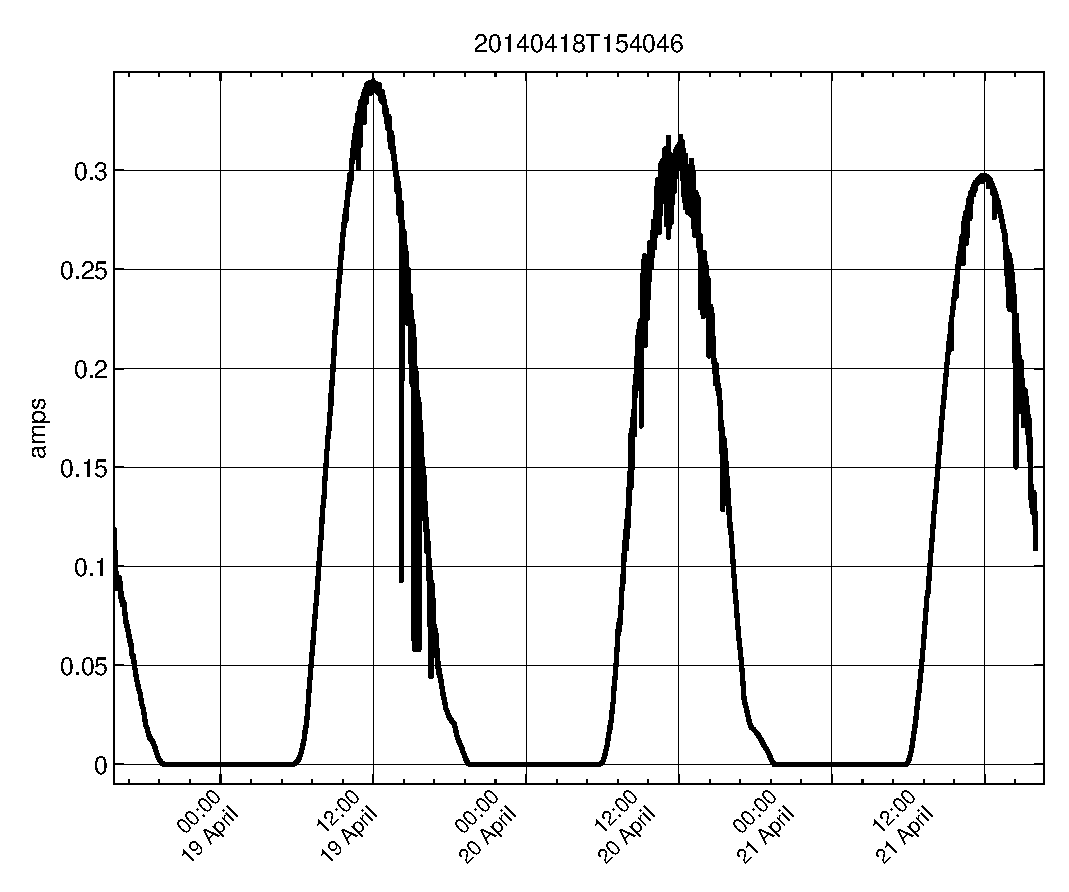
\includegraphics[width = \textwidth]{WESLEY_solar.eps}
\caption{\textit{Current output of 5W solar panel}}
\label{fig:solar}
\end{figure}